\documentclass{book}

% \usepackage[utf8]{inputenc}
\usepackage{polyglossia}
\usepackage[a4paper, landscape, margin=2cm, twoside, bindingoffset=1cm]{geometry}
\usepackage{multicol}
\usepackage[labelformat=simple]{subfig}
\usepackage{graphicx} % showframe
\usepackage{lipsum}
\usepackage{verbatim}
\usepackage{eso-pic}
\usepackage{fancyhdr}
\usepackage{tikz}
\usepackage{titlesec}
\usepackage{xfrac}
\usepackage{pdfpages}
\usepackage{forloop}
\usepackage[export]{adjustbox}
\usepackage{caption}
\usepackage{csquotes}
\usepackage{threeparttable}
\usepackage{longtable}
\usepackage{floatpag}

\setdefaultlanguage[variant=swiss]{german}

\titleformat{\part}{\normalfont\Huge\bfseries}{}{0em}{}
\titleformat{\chapter}{\normalfont\huge\bfseries}{}{0em}{}
\titleformat{\section}{\normalfont\Large\bfseries}{}{0em}{}
\titleformat{\subsection}{\normalfont\large\bfseries}{}{0em}{}
\titleformat{\subsubsection}{\normalfont\normalsize\bfseries}{}{0em}{}
\titleformat{\paragraph}[runin]{\normalfont\normalsize\bfseries}{}{0em}{}
\titleformat{\subparagraph}[runin]{\normalfont\normalsize\bfseries}{0}{0em}{}

\titlespacing{\chapter}{0em}{0em}{0em}


% redefine plain style (used by first pages of chapters)
\fancypagestyle{plain}{
    \lhead{}
    \fancyhead{}
    \fancyfoot{}
    \renewcommand{\headrulewidth}{0pt}
}

\fancyhf{}
\fancyhead[RO]{\leftmark{}}
\fancyhead[LE]{\leftmark{}}
\fancyfoot[RO]{\thepage}
\fancyfoot[LE]{\thepage}
\pagestyle{fancy}
\floatpagestyle{fancy}

\renewcommand{\headrulewidth}{0pt}
\renewcommand{\chaptermark}[1]{\markboth{#1}{}}
\renewcommand{\sectionmark}[1]{\markboth{#1}{}}
\renewcommand{\subsectionmark}[1]{\markboth{#1}{}}

\renewcommand{\thesubfigure}{\relax}  % Do nothing for the counter »subfigure«


\setlength\columnsep{1cm} %distance between multicolumn columns
\captionsetup{font=small, labelformat=empty} % Bildtitel ohne Kapitelangabe
\captionsetup[subfigure]{justification=justified,singlelinecheck=false}

\newcommand{\groupphoto}[4][0.8]{
    {
            \captionsetup{singlelinecheck=false} % left aligned
            \begin{figure}[!htbp]
                \thisfloatpagestyle{empty}
                \centering
                \def\theight{#1}
                \begin{measuredfigure}
                    \includegraphics[width=0.93\textwidth,height=\theight\textheight, keepaspectratio]{#2}
                \end{measuredfigure}
                \caption{#3}
                \label{#4}
            \end{figure}
        }
}

\newcommand{\portrait}[3][0.8]{
    {
            \captionsetup{singlelinecheck=false} % left aligned
            \begin{figure}[!htbp]
                \def\theight{#1}
                \begin{measuredfigure}
                    \includegraphics[width=0.93\textwidth, height=\theight\textheight, keepaspectratio]{#2}
                    \caption{#3}
                \end{measuredfigure}
            \end{figure}
        }
}
\newcommand{\ConcertProg}[2][0.8]{{
            \begin{figure}[!htbp]
                \centering
                \def\theight{#1}
                \includegraphics[height=\theight\textheight,keepaspectratio]{#2}%
            \end{figure}
        }}

\newcommand{\ConcertProgsTwoVertical}[3][0.485]{{
            \begin{figure}[!htbp]
                \centering
                \def\theight{#1}
                \subfloat{%
                    \includegraphics[height=\theight\textheight,keepaspectratio]{#2}%
                }\\
                \subfloat{%
                    \includegraphics[height=\theight\textheight,keepaspectratio]{#3}%
                }
            \end{figure}
        }}

\newcommand{\ConcertProgsTwoHorizontal}[3][0.485]{{
            \begin{figure}[!htbp]
                \centering
                \def\twidth{#1}
                \subfloat{%
                    \includegraphics[height=\twidth\textwidth,keepaspectratio]{#2}%
                }\hfil
                \subfloat{%
                    \includegraphics[height=\twidth\textwidth,keepaspectratio]{#3}%
                }
            \end{figure}
        }}

\newcommand{\ConcertProgsFourOnPage}[5][0.47]{{
            \begin{figure}[!htbp]
                \centering
                \def\theight{#1}
                \subfloat{%
                    \includegraphics[height=\theight\textheight,keepaspectratio]{#2}%
                }\hfil
                \subfloat{%
                    \includegraphics[height=\theight\textheight,keepaspectratio]{#3}%
                }\\
                \subfloat{%
                    \includegraphics[height=\theight\textheight,keepaspectratio]{#4}%
                }\hfil
                \subfloat{%
                    \includegraphics[height=\theight\textheight,keepaspectratio]{#5}%
                }
            \end{figure}
        }}

\newenvironment{history}{\begin{multicols}{2}}{\end{multicols}} % multicolumn for history text





\chapter{Die ersten Jahre}
\input{./chap/Gruendung.tex}
\begin{multicols}{2}

    \subsection{Statuten vom 25. März 1876}

    Es hat sich in der Gemeinde Hildisrieden unter obigem
    Datum eine neue Musikgesellschaft gebildet, welche
    den Mitgliedern zum besseren Gedeihen der Gesellschaft
    folgende Bedingungen festgesetzt:

    \S1
    Jedes Mitglied soll, wenn möglich, lange bei der Gesellschaft
    verbleiben und dieselbe fördern.

    \S2
    Die Gesellschaft bildet sich nicht nur zum Schein, sie
    will auch etwas erlernen, um sich auch produzieren zu
    können, daher verpflichtet sich jedes Mitglied, an den
    vorhergesagten Proben zu erscheinen.

    \S3
    Zum Bestimmen der Proben, sowie zum Dirigieren
    wählt die Gesellschaft einen Kapellmeister.

    \S4
    Wer an der Probe 20 Minuten zu spät erscheint, der
    wird um 20 Cts., wer eine halbe Stunde zu spät kommt
    um 30, und wer gar nicht erscheint, um 50 Cts. bestraft.

    \S5
    Wenn es gewisse Umstände verlangen, so ist der Kapellmeister
    berechtigt, festzustellen, was von den Mitgliedern bis zur
    nächsten Probe gelernt werden soll.

    \S6
    Wird etwas nicht gelernt und man sieht, dass es flissentlich
    nicht geschehen ist, so ist der Betreffende in
    eine Strafe von 30 Cts. verfallen, die jedoch auch erhöht werden
    kann bis auf einen Franken.

    \S7
    Kann sich ein Mitglied mit der Gesellschaft nicht mehr
    vertragen, so steht es dieser frei, das Mitglied auszuschliessen,

    \S8
    Tritt ein Mitglied nach eigener Willkür aus der Gesellschaft,
    so hat es eine Entschädigung von 20 Fr. zu entrichten.

    \S9
    Wer nicht mehr an den Proben erscheint, der schliesst
    sich von selbst aus der Gesellschaft und die Entschädigung folgt.
    Die Gelder, Strafgelder sowie andere, sind vom Präsidenten einzuziehen
    und er hat die Pflicht, zu besorgen und am Ende des Jahres oder wenn
    es die Gesellschaft verlangt, genaue Rechnung abzugeben.

    \S10 |
    Was Instrumente anbetrifft, so hat jedes Mitglied das
    seinige selbst anzuschaffen und zu besorgen. Ein
    schlechtes Instrument wird nicht geduldet.

    \S12
    Wenn 2/3 der Mitglieder einen Ausmarsch verlangen,
    und ein Mitglied will oder kann nicht kommen, so hat
    es dieser sofort dem Kapellmeister anzuzeigen, sonst
    ist es in eine Strafe von drei Fr. verfallen. Die Gesellschaft
    zieht dann eine andere Person zu und das betreffende Mitglied
    hat selbe zu entschädigen und ihr sein Instrument zu leihen.

    \S13
    Jedes Mitglied soll sich dem Befehl des Kapellmeisters
    und Präsidenten fügen soweit ihnen die Gesellschaft
    das Recht in die Hand gelegt hat.

    \S14
    Kommt etwas vor, das in dem Rechte dieser zwei Personen liegt,
    so wird die Gesellschaft angefragt, und es wird abgestimmt.

    \S15
    Tritt ein neues Mitglied in die Gesellschaft, so hat es eine
    Eintrittszahlung von zehn Fr. zu entrichten und sein Instrument
    anzuschaffen. Dann tritt es in die gleichen Rechte wie die andern Mitglieder.

    \S16
    Auch diese, so wie alle andern Gelder werden vom Präsidenten
    bezogen und er hat am Ende des Jahres genaue Rechnung abzugeben,
    wonach die Gelder unter die Mitglieder gleichmässig verteilt werden.
    Am Ende Jahres hat jedoch ein Saldo von 20 Fr. in der Kasse
    zu bleiben, das zum Anschaffen neuer Musikstücke
    aufs folgende Jahr verwendet wird.

    \S17
    Die Musikstücke werden vom Präsidenten oder Kapellmeister bestellt, sie
    haben jedoch die Gesellschaft zuerst anzufragen.

    \S18
    Die bestellten Stücke werden vom Präsidenten bezahlt
    und er hat darüber Rechnung zu geben.

    \S19
    Würde es der Fall sein, dass ein Mitglied stürbe, so
    würde die Gesellschaft für dasselbe einen angemessenen
    Gottesdienst halten lassen,

    \S20
    Wer bei der Musik sein will, muss auch in die Gesellschaft treten.

    \S21
    Die Gesellschaft wählt einen Vorstand von 3 Mit-
    gliedern: Kapellmeister, Präsident und Schreiber auf
    eine Amtsdauer von zwei Jahren.

    \S22
    Der Schreiber schreibt die Stücke und alles, was die
    Gesellschaft beschlägt, wofür er angemessen entschädigt
    wird.

    \S23
    Als Entschuldigung wird in allen Fällen nur Krankheit oder Militärdienst angenommen.

    \S24
    Jedes Mitglied hat sich eigenhändig zu unterzeichnen.\\


\end{multicols}

\begin{figure}[p]
    \centering
    \includegraphics[scale=0.5]{./chap/MGH-Statuten-1874-S1.jpg}
    \label{fig:Statuten-1874}
\end{figure}
\begin{figure}[p]
    \centering
    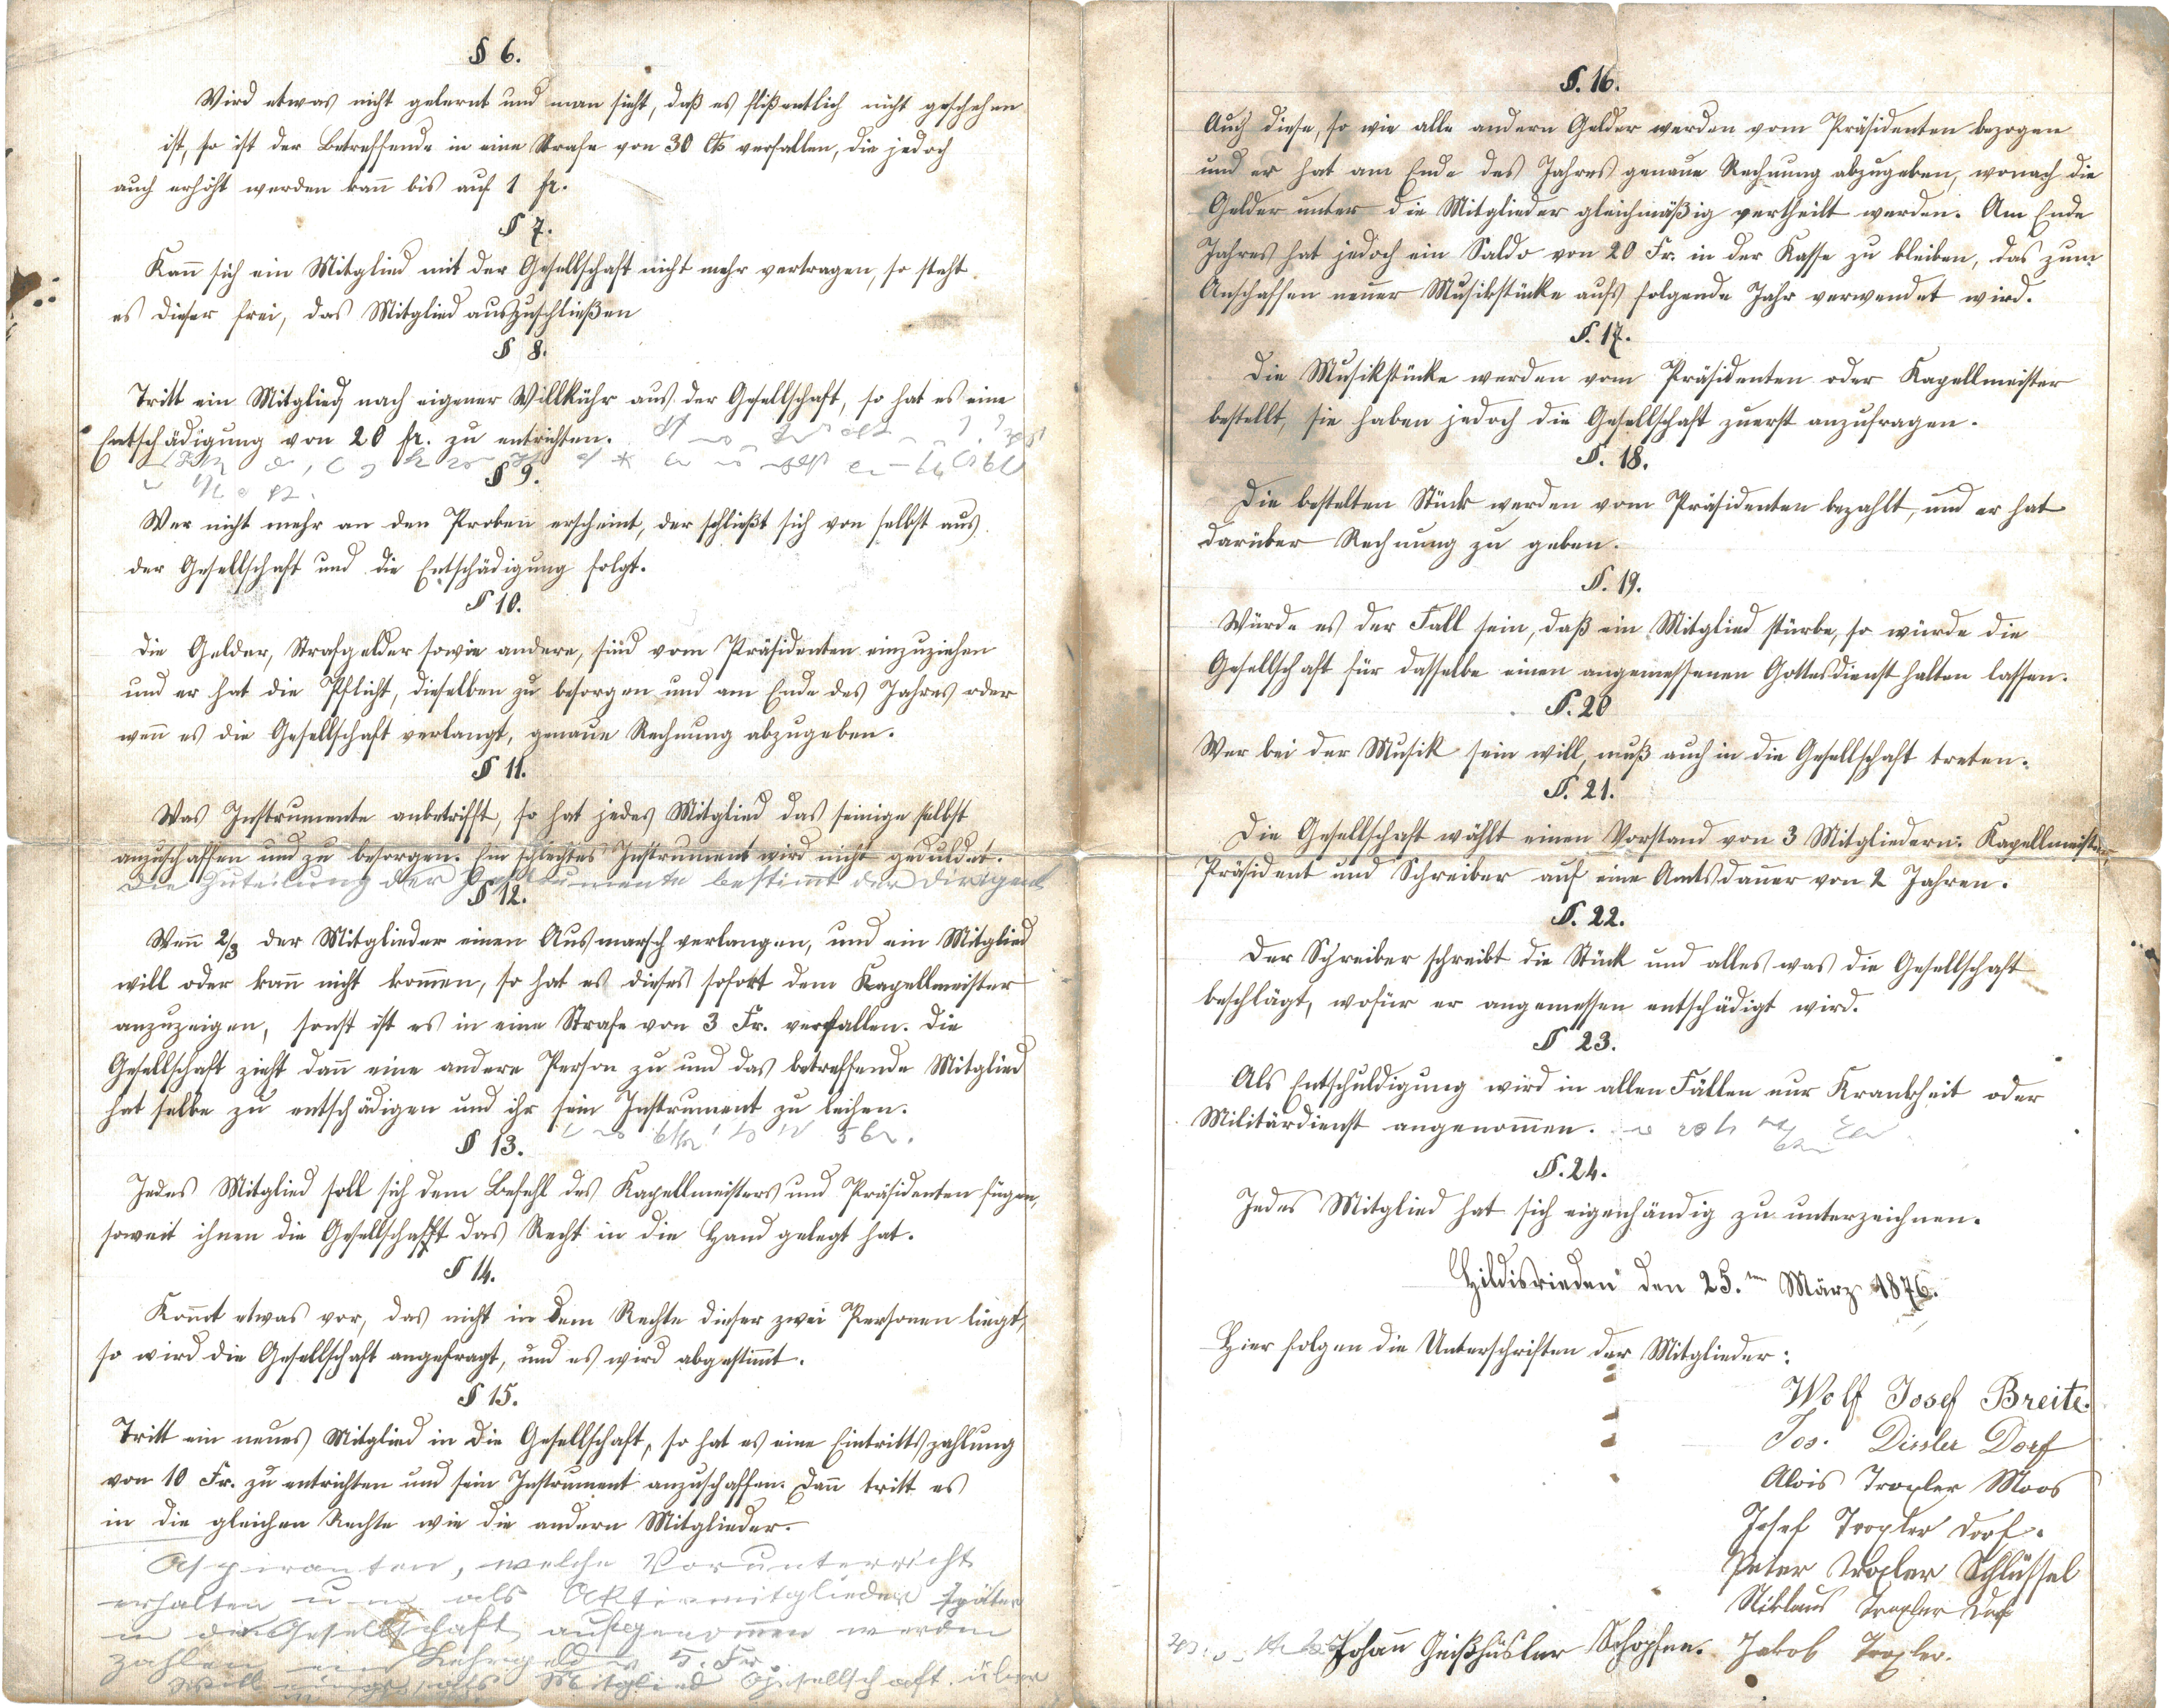
\includegraphics[scale=0.5]{./chap/MGH-Statuten-1874-S2.jpg}
    \label{fig:Statuten-1874}
\end{figure}
\begin{multicols}{2}

    \section{Die Musikgesellschaft Hildisrieden im Jahre 1874}

    1875 — 1900

    Die Wiegenjahre brachten der Musikgesellschaft Hildisrieden abwechslungsreiche Begebenheiten.

    Die Hauptbetätigung blieb weiterhin das Konzertieren in Form von Ständchen und Ausmärschen,
    in- und ausserhalb der Gemeinde, So treffen wir die Musikgesellschaft
    1882 im Emmenbaum anlässlich einer Theateraufführung und 1887 beritten am Auffahrtsumritt in Sempach. Die Entschädigung,
    welche die Musikgesellschaft von der Kirchenverwaltung Sempach erhielt, betrug immerhin 45 Franken. Ein Gesuch, den
    Auffahrtsumritt abwechslungsweise mit der Musikgesellschaft Sempach alle drei Jahre bestreiten zu dürfen, wurde von der Kirchenverwaltung abgelehnt.
    Was unseren Musikanten in den 1890er Jahren vorgeworfen werden konnte,
    war der Mangel an Ordnung    und Disziplin. Wohl hatte man 1884 neue Statuten
    aufgestellt und neue Strafbestimmungen festgesetzt; diese sind aber nicht
    von allen befolgt worden. Diese unruhigen Vereinsjahre, fünf an der Zahl,
    hatten zur Folge, dass man mit dem Gedanken spielte, die Musikgesellschaft
    aufzulösen oder sich den gegebenen Statuten zu fügen.

    Man fand sich hin und wieder zusammen und kam
    ebenso schnell wieder auseinander, bis schliesslich die
    Vernunft siegte. Ein weiterer Grund, der den Zusammenhang des
    Vereins trübte, war der kleine finanzielle Beitrag der Gemeinde.
    Jährlich 20 Franken waren wirklich kein grosses Honorar, wenn man bedenkt,
    dass jeder Musikant sein Instrument selbst zu beschaffen und
    die Musikgesellschaft an sämtlichen Prozessionen teilzunehmen hatte.

    Im Jahre 1899 wurde das Restaurant Kreuz eröffnet und der Saal
    im «Löwen» eingeweiht. Die Einladung zu diesen Festen fügte das
    schwache Gebilde wieder zusammen.

    Die Statuten von 1874 und 1884 erneuert, haben 10
    Mitglieder unterzeichnet. Es sind: Silvester Schnieper,
    Josef Wolf, Leonz Geisshüsler, Silvester Disler, Josef
    Disler, Peter Troxler, Peter Muff, Rudolf Bühlmann,
    Josef Wolf und Niklaus Süess.

    Weitere Einnahmen wurden mit dem «Umblasen»  während der Weihnachtszeit
    in der Gemeinde erzielt. Vor den Häusern wurde jeweils musiziert, wofür die
    Musik-freundlichen Bewohner eine Geldgabe spendeten.
    Im Jahre 1886 brachte der Verein auf diese Weise Fr. 259.60 zusammen.
    Bei kaltem Wetter war das Musizieren kein Vergnügen, denn öfters froren
    die Ventile ein und mussten durch Einhauchen wieder beweglich gemacht werden.
    Gerne wurde dann die Einladung angenommen, ins Haus zu kommen.

    In der warmen Stube liess es sich bequemer musizieren, besonders da,
    wo auch «Mittel» gegen trockene Kehlen bereitstanden.
    Allzulange aber durfte die Gastfreundschaft nicht beansprucht werden,
    warteten doch noch viele Einwohner auf den Besuch der Musikanten.
    War aber dann das gesteckte Tagesziel erreicht, wurde
    es mit dem Aufbruch nicht so genau genommen, gar
    wenn es oft etwas Feines zum Beissen gab.

    Leider ist nun auch dieser alte Brauch verschwunden.
    Dass es hin und wieder gemütlich wurde, berichtet
    die Chronik. Als beim Ausflug auf den Napf ein
    Leiterwagen mit Blumen und Girlanden geschmückt
    dem Sempachersee entlang rasselte, löste sich vom
    Wagen ein Rad, sodass ein Musikant nach dem andern
    vom Wagen kippte. Dabei gab es einige defekte
    Instrumente. Diese konnten in Willisau beim Instrumentenmacher Badmann wieder hergestellt werden.
    Die Fahrt führte ins Luthernbad und von da an zu
    Fuss auf den Napf. Dem Bassisten Troxler war das
    Bergsteigen nicht besonders angenehm, denn er soll sich
    damals geäussert haben: «Dass mer au uf ne so ne Morgelandssiech cha go!»



\end{multicols}


\chapter{1900-1924}

\begin{figure}[p]
    \centering
    \includegraphics{./chap/MGH-1905.jpg}
    \label{fig:mgh-1905}
    \caption{1905}
\end{figure}



\chapter{1974-1999}
\newcounter{year}
\forloop{year}{1974}{\value{year} < 2000}%
{%
    \section{\arabic{year}}
    \begin{figure}[p]
        \centerline{\includegraphics[max size={\textwidth}{\textheight},keepaspectratio]{./chap/\arabic{year}/\arabic{year}.pdf}}
    \end{figure}
    \input{./chap/\arabic{year}/Jahresbericht.tex}
}

\chapter{2000-2024}
\forloop{year}{2000}{\value{year} < 2024}%
{%
    \section{\arabic{year}}
    \ifnum\value{year}=2021
    \else
        \begin{figure}[p]
            \centerline{\includegraphics[max size={\textwidth}{\textheight},keepaspectratio]{./chap/\arabic{year}/\arabic{year}.pdf}}
        \end{figure}
    \fi
    \input{./chap/\arabic{year}/Jahresbericht.tex}
}

\end{document}